% !TEX TS-program = PDFLatexBibtex
%&LaTeX
%Greg and Fred's NSF Grant Dec 2014
\documentclass[11pt]{NSFamsart}
\usepackage{latexsym,amsfonts,amsmath,epsfig,multirow}
\usepackage{stackrel,tabularx,mathtools,enumitem,xspace}
\usepackage[numbers]{natbib}
\usepackage{hyperref,accents}
% This package prints the labels in the margin
%\usepackage[notref,notcite]{showkeys}


%\pagestyle{empty}
\thispagestyle{plain}
\pagestyle{plain}

\headsep-0.6in
%\headsep-0.45in

\setlength{\textwidth}{6.5in}
\setlength{\oddsidemargin}{0in}
\setlength{\evensidemargin}{0in}
\textheight9in
%\textheight9.1in

\providecommand{\FJHickernell}{Hickernell}
\newcommand{\hI}{\hat{I}}
\newcommand{\hatf}{\hat{f}}
\newcommand{\hatg}{\hat{g}}
\newcommand{\tf}{\tilde{f}}
\newcommand{\tbf}{\tilde{\bff}}
\DeclareMathOperator{\cost}{cost}
\DeclareMathOperator{\loss}{loss}
\DeclareMathOperator{\lof}{lof}
\DeclareMathOperator{\reg}{reg}
\DeclareMathOperator{\CV}{CV}

\def\reals{{\mathbb{R}}}
\def\field{{\mathbb{F}}}
\def\complex{{\mathbb{C}}}
\def\naturals{{\mathbb{N}}}
\def\integer{{\mathbb{Z}}}
\def\expect{{\mathbb{E}}}
\def\il{\left<}
\def\ir{\right>}
\def\e{\varepsilon}
\def\g{\gamma}
\def\l{\lambda}
\def\b{\beta}
\def\a{\alpha}
\def\lall{\Lambda^{{\rm all}}}
\def\lstd{\Lambda^{{\rm std}}}

\newcommand{\bbE}{\mathbb{E}}
\newcommand{\tQ}{\widetilde{Q}}
\newcommand{\mA}{\mathsf{A}}
\newcommand{\mB}{\mathsf{B}}
\newcommand{\mC}{\mathsf{C}}
\newcommand{\mD}{\mathsf{D}}
\newcommand{\mG}{\mathsf{G}}
\newcommand{\mH}{\mathsf{H}}
\newcommand{\mI}{\mathsf{I}}
\newcommand{\mK}{\mathsf{K}}
\newcommand{\tmK}{\widetilde{\mathsf{K}}}
\newcommand{\mL}{\mathsf{L}}
\newcommand{\mM}{\mathsf{M}}
\newcommand{\mP}{\mathsf{P}}
\newcommand{\mQ}{\mathsf{Q}}
\newcommand{\mR}{\mathsf{R}}
\newcommand{\mX}{\mathsf{X}}
\newcommand{\mPhi}{\mathsf{\Phi}}
\newcommand{\mPsi}{\mathsf{\Psi}}
\newcommand{\mLambda}{\mathsf{\Lambda}}

\DeclareMathOperator{\APP}{APP}
\DeclareMathOperator{\INT}{INT}
\DeclareMathOperator{\app}{app}
\DeclareMathOperator{\integ}{int}
\DeclareMathOperator{\hAPP}{\widehat{\APP}}
\DeclareMathOperator{\hINT}{\widehat{\INT}}
\DeclareMathOperator{\happ}{\widehat{\app}}
\DeclareMathOperator{\hint}{\widehat{\integ}}
\DeclareMathOperator{\err}{err}
\DeclareMathOperator{\oerr}{\overline{\err}}
\DeclareMathOperator{\apperr}{aerr}
\DeclareMathOperator{\oaerr}{\overline{\apperr}}
\DeclareMathOperator{\interr}{ierr}
\DeclareMathOperator{\oierr}{\overline{\interr}}

\DeclareMathOperator{\Spl}{Spline}
\DeclareMathOperator{\SSpl}{SmSpline}
\DeclareMathOperator{\Power}{Power}
\DeclareMathOperator{\RegSpl}{RegSpline}
\DeclareMathOperator{\MLS}{MLS}
\DeclareMathOperator*{\argmin}{argmin}
\DeclareMathOperator*{\rms}{rms}
\DeclareMathOperator*{\RMSE}{RMSE}
\DeclareMathOperator*{\bias}{bias}
\DeclareMathOperator*{\var}{var}

\newcommand{\bone}{\boldsymbol{1}}
\newcommand{\bzero}{\boldsymbol{0}}
\newcommand{\binf}{\boldsymbol{\infty}}
\newcommand{\ba}{{\boldsymbol{a}}}
\newcommand{\bb}{{\boldsymbol{b}}}
\newcommand{\bc}{{\boldsymbol{c}}}
\newcommand{\bd}{{\boldsymbol{d}}}
\newcommand{\be}{{\boldsymbol{e}}}
\newcommand{\bff}{{\boldsymbol{f}}}
\newcommand{\bhh}{{\boldsymbol{h}}}
\newcommand{\beps}{{\boldsymbol{\varepsilon}}}
\newcommand{\tbeps}{\tilde{\beps}}
\newcommand{\bx}{{\boldsymbol{x}}}
\newcommand{\bX}{{\boldsymbol{X}}}
\newcommand{\bh}{{\boldsymbol{h}}}
\newcommand{\bk}{{\boldsymbol{k}}}
\newcommand{\bg}{{\boldsymbol{g}}}
\newcommand{\bv}{{\boldsymbol{v}}}
\newcommand{\bu}{{\boldsymbol{u}}}
\newcommand{\by}{{\boldsymbol{y}}}
\newcommand{\bt}{{\boldsymbol{t}}}
\newcommand{\bz}{{\boldsymbol{z}}}
\newcommand{\bvarphi}{{\boldsymbol{\varphi}}}
\newcommand{\bgamma}{{\boldsymbol{\gamma}}}
\newcommand{\bphi}{{\boldsymbol{\phi}}}
\newcommand{\bpsi}{{\boldsymbol{\psi}}}
\newcommand{\bnu}{{\boldsymbol{\nu}}}
\newcommand{\balpha}{{\boldsymbol{\alpha}}}
\newcommand{\bbeta}{{\boldsymbol{\beta}}}
\newcommand{\bo}{{\boldsymbol{\omega}}}  %GF added
\newcommand{\newton}[2]{\left(\begin{array}{c} #1\\ #2\end{array}\right)}
\newcommand{\anor}[2]{\| #1\|_{\mu_{#2}}}
\newcommand{\satop}[2]{\stackrel{\scriptstyle{#1}}{\scriptstyle{#2}}}
\newcommand{\setu}{{\mathfrak{u}}}

\newcommand{\me}{\textup{e}}
\newcommand{\mi}{\textup{i}}
\def\d{\textup{d}}
\def\dif{\textup{d}}
%\def\d{{\rm d}}

\def\eavg{{\rm error^{avg}}}
\def\ewc{{\rm error^{wor}}}
\def\ewcavg{{\rm error^{\left\{\substack{\rm wor \\ \rm avg}\right\}}}}
\def\eran{{\rm error^{ran}}}
%\newcommand{\cl}{{\mathfrak{L}}}
\newcommand{\cc}{\mathcal{C}}
\newcommand{\cb}{\mathcal{B}}
\newcommand{\cl}{L}
\newcommand{\cx}{{\Omega}}
\newcommand{\calc}{{\mathcal{C}}}
\newcommand{\calf}{{\mathcal{F}}}
\newcommand{\calfd}{{\calf_d}}
\newcommand{\calh}{{\mathcal{H}}}
\newcommand{\tcalh}{{\widetilde{\calh}}}
\newcommand{\calhk}{\calh_d(K)}
\newcommand{\calg}{{\mathcal{G}}}
\newcommand{\calgd}{{\calg_d}}
\newcommand{\cL}{\mathcal{L}}
\newcommand{\cP}{\mathcal{P}}
\newcommand{\cT}{\mathcal{T}}
\newcommand{\cK}{\mathcal{K}}
\newcommand{\fA}{\mathfrak{A}}
\newcommand{\fC}{\mathfrak{C}}
\newcommand{\fF}{\mathfrak{F}}
\newcommand{\fL}{\mathfrak{L}}
\newcommand{\hS}{\widehat{S}}
\DeclareMathOperator{\Prob}{\mathbb{P}}

\def\abs#1{\ensuremath{\left \lvert #1 \right \rvert}}
\newcommand{\bigabs}[1]{\ensuremath{\bigl \lvert #1 \bigr \rvert}}
\newcommand{\norm}[2][{}]{\ensuremath{\left \lVert #2 \right \rVert}_{#1}}
\newcommand{\ip}[3][{}]{\ensuremath{\left \langle #2, #3 \right \rangle_{#1}}}
\newcommand{\bignorm}[2][{}]{\ensuremath{\bigl \lVert #2 \bigr \rVert}_{#1}}
\newcommand{\calm}{{\mathfrak{M}}}
\DeclareMathOperator{\diag}{diag}
\DeclareMathOperator{\dist}{dist}
\DeclareMathOperator{\filldis}{fill}
\DeclareMathOperator{\sep}{sep}
\DeclareMathOperator{\avg}{avg}
\DeclareMathOperator{\vol}{vol}
\DeclareMathOperator{\cov}{cov}

\newcommand{\des}{\{\bx_i\}}
\newcommand{\desinf}{\{\bx_i\}_{i=1}^{\infty}}
\newcommand{\desn}{\{\bx_i\}_{i=1}^N}
\newcommand{\wts}{\{g_i\}_{i=1}^N}
\newcommand{\wtsn}{\{g_i\}_{i=1}^N}
\newcommand{\datan}{\{y_i\}_{i=1}^N}

%FJH added
\newcommand{\Order}{\mathcal{O}}
\newcommand{\ch}{\mathcal{H}}
\newcommand{\tch}{{\widetilde{\ch}}}
\newcommand{\veps}{\boldsymbol{\varepsilon}}
\DeclareMathOperator{\best}{best}
\newcommand{\hmu}{\hat{\mu}}
\newcommand{\hsigma}{\hat{\sigma}}
\newcommand{\tK}{\widetilde{K}}
\newcommand{\Matlab}{{\sc Matlab}\xspace}
\newcommand{\abstol}{\varepsilon_{\text{a}}}
\newcommand{\reltol}{\varepsilon_{\text{r}}}

\newcommand\starred[1]{\accentset{\star}{#1}}

\newtheorem{resproblem}{Research Problem}
\newtheorem{research}{Research Objectives}

\newcommand{\refproba}{\hyperref[SectHSSVD]{Research Project~1}\xspace}
\newcommand{\refprobaa}{\hyperref[AnalyticEigensubsec]{Research Project~1.1}\xspace}
\newcommand{\refprobab}{\hyperref[NumerEigensubsec]{Research Project~1.2}\xspace}
\newcommand{\refprobac}{\hyperref[SectDesignerKernels]{Research Project~1.3}\xspace}

\newcommand{\refprobb}{\hyperref[SectGAIL]{Research Project~2}\xspace}
\newcommand{\refprobba}{\hyperref[Integrationsubsec]{Research Project~2.1}\xspace}
\newcommand{\refprobbb}{\hyperref[Higherordersubsec]{Research Project~2.2}\xspace}

\newcommand{\refprobc}{\hyperref[combinesec]{Research Project~3}\xspace}
\newcommand{\refprobca}{\hyperref[errestsubsec]{Research Project~3.1}\xspace}
\newcommand{\refprobcb}{\hyperref[parestsubsec]{Research Project~3.2}\xspace}
\newcommand{\refprobcc}{\hyperref[designsubsec]{Research Project~3.3}\xspace}

\newcommand{\refprobd}{\hyperref[appsec]{Research Project~4}\xspace}
\newcommand{\refprobda}{\hyperref[PDEsubsec]{Research Project~4.1}\xspace}
\newcommand{\refprobdb}{\hyperref[SectMEEG]{Research Project~4.2}\xspace}
\newcommand{\refprobdc}{\hyperref[ebolasubsec]{Research Project~4.3}\xspace}
\newcommand{\refprobdd}{\hyperref[Sec_TruncHS]{Research Project~4.4}\xspace}


%\setcounter{page}{1}


\begin{document}
%\setlength{\leftmargini}{2.5ex}

\centerline{\Large \bf Project Description}
\section{Scientific Context and Timeliness of the Proposed Research}
For a long time, scientific research was classified as being either theoretical or experimental in nature. More recently, however, computer simulation (or computer experimentation) has emerged as a third pillar of science \citep{PITAC05,OdenGhattas14}. Sometimes computer experimentation is the only way to obtain an understanding of a physical process, and sometimes it is just considerably cheaper, safer, ethically more responsible or environmentally friendlier than performing an actual physical experiment.
Computer simulation arises quite naturally in situations where one has a complex mathematical model (e.g., specified in terms of a system of partial differential equations or involving randomness) and one can use a computational approach to produce an output (or response) based on a given set of initial conditions and/or model parameters. A few typical examples of where computer simulations are employed are weather and climate modeling, drug design, financial risk management \citep{Gla03}, and the design of nuclear reactors \citep[Sect.\ 2.4]{Smi14a}.

Computer simulation can be quite costly in terms of computation time and high-performance computing hardware.  The potential cost increases when one wishes to perform uncertainty quantification or sensitivity analysis.  Substantial cost savings can often be realized by constructing inexpensive \emph{surrogate models} from the actual outputs of these complex computer simulations \citep{FangEtAl06,ForEtal09,SantnerWilliamsNotz03}.

The research proposed here focuses primarily on \emph{algorithms for constructing surrogates} that will allow us to quickly and reliably predict the output of the computer simulation for a previously not used combination of input factors with an accuracy guaranteed to lie within a user-specified tolerance.  We want our algorithms to have the following properties:
\begin{description}[leftmargin=2.5ex]
\item[Stability] The computations do not suffer from catastrophic round-off error.

\item[Adaptivity] The algorithms adjust their parameters based on the data they observe---rather than a priori knowledge---to meet the specified error tolerance, and they do so with theoretical guarantees.

\item[Efficiency] The computational cost of the algorithms are asymptotically optimal---compared to the best possible algorithms---as the error tolerance vanishes.
\end{description}

In addition to surrogate construction---essentially a problem of function approximation---we will also research two related problems.  One is integration, a simpler problem that shares many of the same mathematical features of function approximation.  Moreover, we will also propose the use of kernels for the numerical solution of PDEs \citep{ChenEtAl14,FornbergFlyer15,SarraKansa09}.

%For the surrogate construction problem, each data point consists of a combination of the input parameters and the corresponding output value. In other words, one needs to run the computer simulation multiple times in order to produce a set of data, and then one can use a function approximation algorithm to produce a response surface which in turn can be evaluated stably, efficiently and accurately for any desired set of input parameters. The number of these input parameters determines the dimensionality of the data fitting problem, and it is not difficult to imagine that this dimension can be rather large. {\bf [Fred, can you add a similar statement about integration?]}

\section{Overview of Proposed Research}
Kernel methods \citep{Fas07a,SchWen06a,Wen05a} are often viewed as an ideal approach to the function approximation problem, which in turn serves as a fundamental application in the context of scattered data fitting and surrogate modeling, but also for classification and regression approaches in machine learning \citep{HasTibFrie01} and as the starting point for various approaches to the solution of partial differential equations, such as, e.g., pseudospectral collocation methods, partition of unity methods, or RBF-based finite difference methods \citep{Fas07a,FornbergFlyer15}.

In the context of surrogate modeling, we are presented with a (costly) computer simulation which generates an output/response, $y=f(\bx)$, given any input $\bx \in \Omega \subset\reals^d$.  The goal is to construct a surrogate, $\tf$, based on the data $(\bx_1, y_1), \ldots, (\bx_N,y_N)$.  An approach based on kernel methods takes the form
\begin{subequations} \label{rbfapprox}
\begin{equation} \label{rbfform}
\tf(\bx) = \sum_{j=1}^N K(\bx,\bx_j) c_j,
\end{equation}
where $K:\Omega \times \Omega \to \reals$ is a known symmetric, positive definite kernel. One example is the Gaussian (or squared exponential) kernel:
\begin{equation}  \label{gausskernel}
K(\bx,\bt) = \exp\bigl(-\gamma_1^2 (x_1-t_1)^2 - \cdots - \gamma_d^2 (x_d-t_d)^2 \bigr), \quad \bx = (x_1,\ldots,x_d),\ \gamma_1,\ldots,\gamma_d >0,
\end{equation}
but there are also other good choices for the kernel.  In the most-straightforward variant, the unknown $\bc=(c_1, \ldots, c_N)^T$ is determined by imposing interpolation.  Specifically,
\begin{equation} \label{rbfcoef}
\bc=\mK^{-1} \by, \qquad \mK=\bigl(K(\bx_i,\bx_j)\bigr)_{i,j=1}^N, \quad \by=\bigl(f(\bx_i)\bigr)_{i=1}^N.
\end{equation}
\end{subequations}

This numerical algorithm goes by different names, such as, radial basis function approximation \citep{Buh03a}, scattered data approximation \citep{Wen05a}, meshfree approximation \citep{Fas07a}, and kriging \citep{Ste99}. It is part of the JMP \citep{JMP11}, \Matlab \citep{MAT8.4} and R \citep{R3.03_2013} software packages.  It is flexible because the data sites need not follow a regular pattern. There is a deterministic optimality: $\tf$ is the best approximation to $f$ in the Hilbert space whose reproducing kernel is $K$ \citep{Fas07a,Wen05a}.  There is a stochastic optimality: $\tf$ is the best approximation to $f$ in the set of Gaussian stochastic processes whose covariance kernel is $K$ \citep{BerT-A04,Wah90}.  The procedure outlined above can be extended to include the exact reproduction of polynomials and also the situation where the $y_i$ are noisy observations of the $f(\bx_i)$ \citep{Wah90}.
One of the main accomplishments of \emph{NSF-DMS-1115392 Kernel Methods for Numerical Computation} (see Sect.~\ref{SectPrevious}) was the development of the so-called \emph{Hilbert--Schmidt SVD} \citep{CavorettoEtAl14,FMcC12,McCF14,McCourtFas14} (see \refproba). This algorithm provides a framework for finding a new stable basis for often ill-conditioned kernel methods.
A second major accomplishment was the development of \emph{guaranteed, adaptive numerical integration algorithms} \citep{HicEtal14b,HicEtal14a,HicJim16a,JimHic16a} (see \refprobb).

Building upon these previous research accomplishments, we propose to extend our work in several different directions:

\begin{description}[leftmargin=2.5ex]

\item[\refproba] Extend our research on the Hilbert--Schmidt SVD by identifying more kernels and their Mercer series for which the Hilbert--Schmidt SVD can be implemented.
\begin{enumerate}
\renewcommand{\labelenumi}{1.\arabic{enumi}.}
\item Analytically compute eigenvalues and eigenfunctions for new kernels $K$.
\item Numerically compute eigenvalues and eigenfunctions for new kernels $K$.
\item Build \emph{designer kernels}, $K$, starting from a given orthogonal set of functions $\{\varphi_n\}_{n=1}^\infty$ and appropriately decaying scalars $\{\lambda_n\}_{n=1}^\infty$ which will serve as eigenfunctions and eigenvalues for $K$.
\end{enumerate}

\item[\refprobb] Extend our research on guaranteed, adaptive algorithms.
\begin{enumerate}
\renewcommand{\labelenumi}{2.\arabic{enumi}.}
\item Develop adaptive (quasi-)Monte Carlo methods for multivariate integration that satisfy both absolute and relative error tolerances.
\item Develop adaptive univariate integration and function approximation algorithms that are higher order and locally adaptive.
\end{enumerate}

\item[\refprobc] Obtain guaranteed, adaptive algorithms for kernel methods.
\begin{enumerate}
\renewcommand{\labelenumi}{3.\arabic{enumi}.}
\item Use cones to obtain error bounds and guarantees for function approximation with kernels.
\item Use the Hilbert--Schmidt SVD for adaptive data-driven parameter estimation of kernel methods.
\item Use the Hilbert--Schmidt SVD to obtain ``optimal'' adaptive data-driven designs for kernel methods.
\end{enumerate}

\item[\refprobd] Apply new results.
\begin{enumerate}
\renewcommand{\labelenumi}{4.\arabic{enumi}.}
\item Use kernel methods and the Hilbert--Schmidt SVD for the solution of PDEs via so-called RBF-(W)ENO (weighted essentially non-oscillatory) methods.
\item Use kernel methods for the solution of the MEG/EEG forward problem.
\item Use kernel methods to create a surrogate model to predict the spread of Ebola in West Africa.
%\item Use the eigenfunction expansion of kernels for low-rank approximations in machine learning.
\end{enumerate}
\end{description}
In the following sections we outline our plans for completing these four projects.

\section*{Research Project 1. Extensions of the Hilbert--Schmidt SVD}\label{SectHSSVD}

Every positive definite kernel $K$ has a Hilbert--Schmidt (or Mercer) series decomposition \citep{CourantHilbert53,RasWil06a}
\begin{equation}\label{HSseries}
K(\bx,\bt) = \sum_{n=1}^\infty \lambda_n \varphi_n(\bx) \varphi_n(\bt),
\end{equation}
where the $\lambda_n$ and $\varphi_n$ are the eigenvalues and eigenfunctions of the associated Hilbert--Schmidt integral operator $\cK : L_2(\Omega, \rho) \to L_2(\Omega, \rho)$ which depends on the probability density $\rho$ and is defined by
\begin{equation}\label{TK}
(\cK f)(\bx) = \int_\Omega K(\bx, \bt)f(\bt)\, \rho(\bt)\, \d \bt.
\end{equation}

The Hilbert--Schmidt SVD \citep{CavorettoEtAl14,FMcC12} of the kernel matrix $\mK$ from \eqref{rbfcoef} is the \emph{formal decomposition}
\begin{subequations}\label{HSSVD}
\begin{equation}
\mK = \mPsi \mLambda_1 \mPhi_1^T,
\end{equation}
where all matrices are of size $N\times N$, but the matrix $\mPsi$ is formed as a product of semi-infinite and bi-infinite matrices, i.e.,
\begin{equation}\label{PsiMatrix}
\mPsi = \left(\mPhi_1\ \mPhi_2\right)\left(\begin{matrix}\mI_N\\\mLambda_2\mPhi_2^T\mPhi_1^{-T}\mLambda_1^{-1}\end{matrix}\right),
\quad
\left(\begin{matrix}\mLambda_1 & \\ & \mLambda_2\end{matrix}\right) = \text{diag}(\lambda_n)_{n=1}^\infty,\ \left(\mPhi_1\ \mPhi_2\right) = \mPhi = \left(\varphi_n(\bx_i)\right)_{i,n=1}^{N,\infty}.
\end{equation}
\end{subequations}
For practical applications the matrices $\mLambda_2$ and $\mPhi_2$ will therefore have to be truncated appropriately \citep{CavorettoEtAl14,FMcC12}.
We refer to the Hilbert--Schmidt SVD \eqref{HSSVD} as a ``formal decomposition'' since it is important to note that the matrices $\mPsi$, $\mLambda_1$, $\mLambda_2$, $\mPhi_1$ and $\mPhi_2$ are not found by manipulating $\mK$, but are formed directly from the eigenvalues and eigenfunctions of $\cK$. In fact, \emph{the ill-conditioned matrix $\mK$ never needs to be formed, nor is precise knowledge of the closed form of the kernel $K$ essential}. As long as the eigenfunctions and eigenvalues are known, the Hilbert--Schmidt SVD enables us to formulate stable and efficient algorithms for the associated kernel approximation problems \citep{CavorettoEtAl14}. These insights are the motivation for \refprobaa--\refprobac.

From \eqref{PsiMatrix} we see that the Hilbert--Schmidt SVD provides a new and stable basis $\{\psi_1,\ldots,\psi_N\}$ collected in the vector
\begin{equation}\label{StableBasis}
\bpsi(\cdot)^T = \bphi(\cdot)^T\left(\begin{matrix}\mI_N\\\mLambda_2\mPhi_2^T\mPhi_1^{-T}\mLambda_1^{-1}\end{matrix}\right),
\end{equation}
which can be viewed as a generic row of $\mPsi$. This serves as an alternative to the standard basis $\{K(\cdot,\bx_1),\ldots,K(\cdot,\bx_N)\}$ collected in the vector $\bk(\cdot)^T = \bpsi(\cdot)^T\mLambda_1\mPhi_1^T$, where $\bphi(\cdot)^T$ is a vector of eigenfunctions. If we apply the Hilbert--Schmidt SVD to the standard (or direct) interpolation approach \eqref{rbfapprox} then the result is a stable linear system of the form $\mPsi \bb = \by$, and the interpolant is evaluated as $\tf(\bx) = \sum_{j=1}^N \psi_j(\bx) b_j = \bpsi(\bx)^T \bb$.

A typical comparison between interpolation errors based on the standard approach and the Hilbert--Schmidt approach for isotropic Gaussian kernel interpolation is shown in the left plot of Fig.~\ref{Fig_HSSVD}. The most accurate results are obtained for a positive value of $\gamma$, and they compare favorably to a polynomial interpolant corresponding to the ``flat'' $\gamma\to0$ limit. Moreover, in or near the ``flat'' limit regime the standard approach generates completely unreliable results (the dashed lines), i.e., the standard approach yields reliable answers only for relatively spiky kernels.

\begin{figure}[h]
    \centering
    \includegraphics[width=.4\linewidth]{Fig_Error_ex17j}
    \includegraphics[width=.4\linewidth]{Fig_MLE_ex17j}
\caption{Interpolation errors (left) and maximum likelihood estimates of ``optimal'' $\gamma$ (right) for data sampled at $N$ Halton points from $f(\bx) = \sin\left(\tfrac{x_1+x_2+\ldots+x_5}{5}\right)$, $\bx=(x_1,x_2,\ldots,x_5) \in [-1,1]^5$. Solid lines denote Hilbert--Schmidt SVD, dashed lines standard basis approach.}\label{Fig_HSSVD}
\end{figure}

While Fig.~\ref{Fig_HSSVD} demonstrates that we are able to solve simple moderate-dimensional problems, the results of \cite{FasHicWoz12b, FasHicWoz12a} show that the use of anisotropic kernels is essential for maintaining good convergence rates in high dimensions. Therefore, in addition to the research projects we are about to describe, the implementation of the Hilbert--Schmidt SVD algorithm needs to be extended to the anisotropic case.

\subsection*{Research Project 1.1. Analytical Computation of Eigensystems} \label{AnalyticEigensubsec}

In addition to the Gaussian kernel \citep{FMcC12} and the iterated Brownian bridge kernels \citep{CavorettoEtAl14}, there are many other kernels for which it would be desirable to have stable and reliable algorithms. One family of special interest in the statistics community \citep{Ste99} are the Mat\'ern kernels defined on $\reals^d$, $K(\bx,\bt) = K_{\beta-d/2}\left(\gamma\|\bx-\bt\|\right) \left( \gamma \| \bx - \bt \|\right)^{\beta-d/2}$, $\beta > \frac d2$,
where $K_{\beta-d/2}$ are modified Bessel functions of the second kind and $\beta$ is a smoothness parameter that should be chosen in a data-dependent way together with the shape parameter $\gamma$. For $\beta = \frac{d + 2k+1}{2}$, $k=0,1,2,\ldots$, the Mat\'ern kernels take on a simpler form. For example
\begin{subequations}\label{Maternkernels}
\begin{align}
\text{$k = 0$, i.e., $\beta = \frac{d+1}{2}$:}\quad & K(\bx,\bt) = \me^{-\gamma \|\bx-\bt\|}, \label{C0Matern} \\
\text{$k = 1$, i.e., $\beta = \frac{d+3}{2}$:}\quad & K(\bx,\bt) = (1+\gamma \|\bx-\bt\|)\me^{-\gamma \|\bx-\bt\|}, \label{C2Matern}\\
\text{$k = 2$, i.e., $\beta = \frac{d+5}{2}$:}\quad & K(\bx,\bt) = \left(1+\gamma \|\bx-\bt\|+\frac{1}{3}(\gamma \|\bx-\bt\|)^2\right)\me^{-\gamma \|\bx-\bt\|}.\label{C4Matern}
\end{align}
\end{subequations}
The integral equation $2\int_0^\infty \me^{-\gamma|x-t|}\varphi(t)\me^{-2t} \dif t = \lambda \varphi(x)$ was solved by \citet{Juncosa45} in the context of random noise in radio receivers. This can be interpreted as the Hilbert--Schmidt integral eigenvalue problem for the $k=0$ Mat\'ern kernel \eqref{C0Matern} on $[0,\infty)$ with $\rho(x) = 2\me^{-2|x|}$. We plan to generalize the work of \citet{Juncosa45} in two steps. First, we plan to obtain the eigenvalues and eigenfunctions of the $k=0$ Mat\'ern kernel on the entire real line. Next, we will tackle Mat\'ern kernels with higher smoothness on $\reals$ by solving the corresponding ODE boundary value problems of increasingly higher order. While a generalization of this approach to higher dimensions seems unlikely, it will be possible to consider product kernels as a new type of designer kernel (see Section \refprobac).

\subsection*{Research Project 1.2. Numerical Computation of Eigensystems} \label{NumerEigensubsec}

The Hilbert--Schmidt SVD depends on the availability of the eigenvalues and eigenfunctions of $\cK$. If the analytical approach in \refprobab\ fails, then we can instead generate approximate eigenvalues and eigenfunctions numerically. This is especially useful if one wants to use ``traditional'' (RBF) kernels such as (inverse) multiquadrics, for which the analytical eigensystems are not known to us. The standard approach to approximating the eigenfunctions of the Hilbert--Schmidt operator $\cK$ uses a Nystr\"om method (see, e.g., \citep{Atkinson97,BachJordan03}). We propose the use of a more general collocation method.
Assuming that the eigenfunctions can be approximated as
$\varphi(\bx) \approx \sum_{j=1}^{N_b} h_j(\bx) d_j$, where $\{h_1,h_2,\ldots,h_{N_b}\}$, is a basis of a finite-dimensional approximation space, one can use $N_c$ collocation points $\bx_1,\ldots,\bx_{N_c}$ to discretize the Hilbert--Schmidt integral eigenvalue problem resulting in a rectangular generalized eigenvalue problem with $N_c\times N_b$ matrices $\mA$ and $\mH$
\begin{equation}\label{GeneralizedEVProblem}
    \mA\bd = \lambda\mH\bd, \qquad \mA_{ij}=\int_\Omega K(\bx_i,\bt) h_j(\bt)\d\bt, \quad \mH_{ij}=h_j(\bx_i).
\end{equation}
Depending on the choice of basis and kernel, it may be possible to evaluate these integrals analytically or not. In the latter case we will use the quadrature rules of \refprobb. Since the solution of \eqref{GeneralizedEVProblem} in its full generality is not yet a standard numerical linear algebra problem---although some work exists \citep{DasNeumaier13}---we will also consider the simpler case when $N_c=N_b$,
%i.e., the number of collocation points equals the number of basis functions,
for which one of the REU students funded by our previous grant has obtained preliminary results. An important advantage of the collocation method over the simpler Nystr\"om method is that we can evaluate the approximate eigenfunctions at any point $\bx \in \Omega$ and therefore we can directly use those functions and corresponding eigenvalues just as we would use the analytical formulas from \refprobaa to fill the matrices involved in the Hilbert--Schmidt SVD. All the advantages of using kernels and the Hilbert--Schmidt SVD will still be available to us, such as optimality, data-dependence (as demanded for higher dimensions by the Mairhuber--Curtis theorem \citep{Fas07a}) and stability.

\subsection*{Research Project 1.3. Designer Kernels}\label{SectDesignerKernels}
In addition to the ``traditional'' approach in which we are given some kernel (such as, e.g., a Gaussian) whose eigensystem we can then use with the Hilbert--Schmidt SVD, it is also possible to turn the picture upside down and build a positive definite kernel via Mercer's theorem by combining an appropriate sequence of
``eigenvalues'' $\{\lambda_n\}_{n=1}^\infty$ with a given set of orthogonal functions. Thus, the closed form of the kernel may or may not be known in this case. For example, one could start with Chebyshev polynomials on $[-1,1]$ and combine them with either a sequence of algebraically or geometrically decaying eigenvalues. This will result in Mercer kernels that provide either algebraic of spectral approximation rates and can be implemented stably and reliably within the Hilbert--Schmidt SVD framework. The iterated Brownian bridge kernels of \cite{CavorettoEtAl14} provide another example of a family of designer kernels where the sinusoidal eigenfunctions (see \eqref{IBBkernel}) were chosen to satisfy boundary conditions generalizing those of natural cubic splines. Kernels with other (e.g., periodic) boundary conditions can be constructed using similar ideas.

\section*{Research Project 2. Extensions of Guaranteed, Adaptive Algorithms}\label{SectGAIL}

In our previous NSF-funded work (see Sect.\ \ref{previousmeritsubsec}) we derived a number of  adaptive algorithms for function approximation and integration, that are \emph{guaranteed} to satisfy the user-specified error tolerance.  This sets them apart from existing adaptive algorithms, which have no such guarantees.  For example, \Matlab's adaptive quadrature algorithm, \texttt{integral}, has no theoretical guarantee of success.  \Matlab has no adaptive (quasi-)Monte Carlo cubature methods (guaranteed or not).  The Chebfun \Matlab toolbox \citep{TrefEtal14} solves a host of problems adaptively, but has no theoretical guarantees.  Our proposed new adaptive algorithms will build upon our previous work and provide guarantees of success, upper bounds on computational cost, and proof of asymptotic optimality.

\subsection*{Research Project 2.1. Adaptive (Quasi-) Monte Carlo Algorithms for Multivariate Integration}\label{Integrationsubsec}
Multivariate integrals may be approximated by an average of function values:
\begin{equation} \label{integprob}
I(f) := \int_{\reals^d} f(\bx)  \, \varrho(\bx) \, \dif \bx \approx
\frac 1 N \sum_{i=1}^N f(\bx_i) =: \hI_N(f).
\end{equation}
Here $\varrho$ is a probability density function, and the well-chosen data sites come from an infinite sequence $\desinf$.  In the applications we have in mind, $f$ is not smooth enough or $d$ is large enough that tensor product rules of higher order are not competitive.  Two popular choices are i) independent and identically distributed (IID) points with density $\varrho$---corresponding to simple Monte Carlo sampling---and ii) suitably transformed low discrepancy sequences, such as digital sequences or integration lattice sequences---corresponding to quasi-Monte Carlo sampling \citep{Nie92,SloJoe94,Lem09a,DicPil10a,DicEtal14a,Owe13a}.

In our previous NSF-funded project we developed a simple Monte Carlo algorithm \citep{HicEtal14b} and two quasi-Monte Carlo algorithms \citep{HicJim16a,JimHic16a}, that \emph{adaptively} choose the sample size, $N$, to satisfy the user-specified error tolerance:
\begin{equation} \label{cubMCguar}
\bigabs{I(f) -\hI_N(f)} \le \abstol \quad \text{or} \quad \Prob\bigl[\bigabs{I(f) -\hI_N(f)} \le \abstol \bigr] \le 1-\alpha,
\end{equation}
the former holding for deterministic quasi-Monte Carlo sampling, and the latter holding for the random simple Monte Carlo sampling and confidence level $1-\alpha$.  All three adaptive algorithms base their decisions on data-driven error estimates, rather than a priori knowledge of the integrands.

We will extend these algorithms to handle a hybrid absolute/relative error tolerance of the form $\max(\abstol,\reltol \abs{I(f)})$, which is more flexible than our present pure absolute error tolerance, $\abstol$.  Since we already know how to estimate the error from the data, this problem is partially solved.  The missing piece is how to estimate $I(f)$ appearing in the error tolerance, $\max(\abstol,\reltol \abs{I(f)})$.  This will require an unspecified number of iterations.  For the simple Monte Carlo algorithm we must ensure that all these iterations combined stay within the specified confidence level.

We also propose to add control variates to our adaptive (quasi-)Monte Carlo algorithms.  Given an integrand $g$ whose integral, $I(g)$, is known, the control variate estimator is $\hI_{\CV,N}=\hI_N(f) + \beta [ I(g) - \hI_N(g)]$.  For simple Monte Carlo sampling there is a standard way to estimate the optimal $\beta$, but this method may give the wrong answer for low discrepancy sampling \citep{HicEtal03}.  We will follow this insight and find a better way of determining $\beta$ for low discrepancy sampling.

Option pricing is an important application of multivariate integration, and the case where the stock price is monitored continuously corresponds to the  limiting case of $d\to \infty$.  Multi-level methods \citep{Hei01a,Gil14a,HicMGRitNiu09a,NiuHic09b} have been found to be successful in efficiently evaluating infinite dimensional integrals.  We will extend our existing adaptive (quasi-)Monte Carlo algorithms to become adaptive multi-level methods.  The unbiased approach of \cite{RheGly12a} looks very promising.

Besides establishing rigorous guarantees for our new algorithms, we also will establish upper bounds on the computational cost of these algorithms.  As in our previous work, the cost depends not only on the known input parameters, such as the error tolerance(s) and the uncertainty, $\alpha$, but also on unknown quantities, such as the variance of $f(\bX)$, $\bX \sim \varrho$ (for simple Monte Carlo) and the rate of decay of the series coefficients for $f$ (for quasi-Monte Carlo).  This is natural since adaptive algorithms by nature expend different amounts of effort depending on the difficulty of the problem.  We also propose to show that these computational costs are asymptotically optimal relative to the best possible algorithms that make the same assumptions on the set of possible integrands.  This will be done by using bump functions, a well-known method in the information-based complexity literature (see \cite{TraWasWoz88,Nov88}).

\subsection*{Research Project 2.2. Higher Order and Locally Adaptive Univariate Function Approximation and Integration}\label{Higherordersubsec}
In our previous NSF-funded project (see Sect.\ \ref{previousmeritsubsec}) we developed adaptive univariate function approximation and integration algorithms based on linear splines, but \emph{with rigorous guarantees of success} \citep{HicEtal14b}.  In our proposed work we will extend these methods in two directions.  One obvious goal is to increase the efficiency by using higher order function approximation than the linear spline. The general framework provided in \cite{HicEtal14b} will facilitate this.

All of our adaptive algorithms for univariate or multivariate problems developed so far have been globally adaptive, i.e., the design, $\desinf$, is fixed but the number of data, $N$, is determined adaptively.  This is called global adaption.  A second goal of this project  is to introduce local adaption, i.e., algorithms where the density of the data sites, as well as their number, depends on the function data.  This is easiest to do for univariate problems.  We will sub-divide the whole domain into sub-domains and solve function approximation or integration problem separately on those.  These subdivisions will be data driven.

Finally, as was done for the original algorithms in\citep{HicEtal14b}, we will derive upper bounds on the costs of our new higher order and locally adaptive algorithms.  We will also demonstrate their asymptotic optimality by using bump functions \cite{TraWasWoz88,Nov88}.

\subsection*{Why Cones} The adaptive algorithms that we have derived in our previous work, and the adaptive algorithms that we propose to derive are or will be \emph{guaranteed} to satisfy the user-specified error tolerance.  This sets them apart from existing adaptive algorithms, which have no such guarantees.  For example, \Matlab's adaptive quadrature algorithm, \texttt{integral}, has no theoretical guarantee of success.  \Matlab has no adaptive (quasi-)Monte Carlo cubature methods (guaranteed or not), and \Matlab's spline functions for univariate function approximation are not adaptive either.

To obtain rigorous guarantees of success for adaptive algorithms requires limiting the functions to some set, $\calc$.  Our past experience and future expectation is that $\calc$ turns out to be a \emph{cone} of functions. There is a good reason for this.

The true absolute error of function approximation or integration, $\err(f,N):=\bignorm[\infty]{f-\tf}$ or $\err(f,N):= \bigabs{I(f) - \hI_N(f)}$, is positively homogeneous, i.e., $\err(cf,N)=\abs{c} \err(f,N)$. So we expect any reasonable data-driven error bound, $\oerr(f,N)$, to also be positively homogeneous.  This means that the set of functions for which the error bound is correct, $\calc:=\{f : \err(f,N) \le \oerr(f,N)\}$, must be a cone, i.e., $f\in \calc \implies cf \in \calc$.

\section*{Research Project 3. Combining Kernel Methods with Guaranteed and Adpative Algorithms} \label{combinesec}

\subsection*{Research Project 3.1. Data-Driven Error Estimation}\label{errestsubsec} Our goal is to construct adaptive meshfree function approximation algorithms.  This requires an error bound, $\oerr(f,N)$, based on the function data, that conservatively estimates the true error, $\err(f,N):=\bignorm[\infty]{f-\tf}$. Cross-validation (CV) is sometimes used to approximate the error. One form of CV is
\begin{subequations} \label{rbferrbd}
\begin{multline} \label{crossvalid}
\err(f,N) \\
\approx \sqrt{\frac{C}{N} \left[ \sum_{i=1}^{N/2} \abs{f(\bx_{2i-1})-\tf(\bx_{2i-1};\{\bx_{2i}\}_{i=1}^{N/2})}^2 + \sum_{i=1}^{N/2} \abs{f(\bx_{2i})-\tf(\bx_{2i};\{\bx_{2i-1}\}_{i=1}^{N/2})}^2 \right]}.
\end{multline}
There also exist rigorous error bounds of the form \citep{Wen05a}
\begin{align}
\label{powfunerrbd}
\err(f,N) & \le \sqrt{\sup_{\bx \in \cx}[K(\bx,\bx)-\bk^T(\bx)\mK^{-1} \bk(\bx)]} \norm[\ch]{f} \\
\label{filldiserrbd}
\err(f,N) & \le C [\filldis(\desn)]^r \norm[\ch]{f}, \qquad
\filldis(\desn): = \sup_{\bx \in \cx} \min_{i=1,  \ldots, N} \norm[2]{\bx - \bx_i}.
\end{align}
\end{subequations}
All of these expressions have drawbacks as candidates for a data-driven $\oerr(f,N)$.  CV has no finite-sample size guarantees of successfully providing an upper bound on the true error.  The error bounds in or (\ref{powfunerrbd}, \ref{filldiserrbd}) require $\norm[\ch]{f}$, which is not known a priori. computation of $\bk^T(\bx)\mK^{-1} \bk(\bx)$ may suffer from stability issues.  Taking the supremums in \ref{powfunerrbd}, \ref{filldiserrbd}) are nontrivial. While $r$ denotes the kernel smoothness in \eqref{filldiserrbd}, the constant $C$ is not always known explicitly.

We propose find guaranteed data-driven error bounds for functions in certain  \emph{cones}.  Given our experience with the integration problem, these cones may take the form of a strong norm of the function being bounded above by a weaker norm, as in \cite{HicEtal14b}.  This may allow us to justify the CV. Alternatively, our cones they may involve assumptions on the regularity of the bases, $\varphi_n$, as in \cite{HicJim16a,JimHic16a} and suggest that we deal directly with the bases---rather than the kernels---in our calculations as in \refproba.  We may find some other way to overcome the drawbacks for one of the error bounds listed above.  For example, the results of \refproba may help us overcome the instablity problem of computing with $\mK^{-1}$.

The Hilbert--Schmidt series of the iterated Brownian bridge kernels \citep{CavorettoEtAl14} is given by
\begin{equation}\label{IBBkernel}
K(x,t) = \sum_{n=1}^{\infty} \left(n^2\pi^2 + \gamma^2\right)^{-\beta} 2\sin(n\pi x) \sin(n\pi t), \quad x,t \in [0,1],\ \gamma>0, \beta \in \mathbb{N},
\end{equation}
and therefore it is a perfect candidate for the data-driven error bounds discussed above since the eigenfunctions do not depend on the parameters $\beta$ and $\gamma$, while a smaller smoothness parameter $\beta$ leads to slower decay of the eigenvalues.

\subsection*{Research Project 3.2. Data-Driven Parameter Estimation} \label{parestsubsec}
Parameters of the kernel $K$---such as the shape parameters $\gamma_\ell>0$ for the anisotropic Gaussian kernel in \eqref{gausskernel}, or the smoothness and shape parameters, $\beta$ and $\gamma$, for the Mat\'ern kernels in \eqref{Maternkernels}---may be estimated by maximum likelihood estimation (MLE).  In practice, one usually assumes that the data is generated by a Gaussian process, and then often uses the profile log-likelihood $\ell(\bgamma) = N\log(\by^T\mK^{-1}\by) + \log(\det(\mK))$ to estimate the ``best'' kernel parameters. Here these parameters are collected in the vector $\bgamma$.  The sample size, $N$, and the vector of given function values, $\by$, are as in \eqref{rbfcoef}. Since the matrix $\mK$, which depends on $\bgamma$, can easily become \emph{ill-conditioned even for moderate $N$} the profile log-likelihood needs to be computed with a stable numerical algorithm such as the Hilbert--Schmidt SVD since it becomes unreliable otherwise (see Fig.~\ref{Fig_HSSVD}).
%The ill-conditioning will arise if the kernel has a high degree of smoothness, and/or if it becomes ``flat'' (the $\gamma_\ell$ are near zero). This means that $f$ is very smooth and the discretization error \eqref{rbferrbd} vanishes rapidly as the fill distance decreases.
As Fig.~\ref{Fig_HSSVD} also shows, for any given set of data, finding an ``optimal'' (or near-optimal) value of the kernel parameter(s) can have a significant impact on the accuracy of the recovered function $\tf$. A number of potential criteria for optimizing kernel parameters were introduced in \citep{Fasshauer11}. However, up to now all of those criteria were based on the use of the standard approach, i.e., they were subject to the effects of ill-conditioning of $\mK$, and thus often unreliable or impractical. Recently, the MLE criterion (or more precisely, profile log-likelihood) was the first of these criteria to be converted to the stable framework \citep{McCourtFas14}, and this is the approach used in the right part of Fig.~\ref{Fig_HSSVD}. We propose to extend the application of the Hilbert--Schmidt SVD to other criteria, and then to investigate which of these criteria is most effective.



\subsection*{Research Project 3.3. Data-Driven Designs} \label{designsubsec}
An important issue is not only the surface fitting problem itself, but also the choice of \emph{design}, i.e., the data locations or input parameter settings. The main objectives for finding a ``good'' design are that it successfully deal with the \emph{curse of dimensionality}, i.e., that it effectively fill out the high-dimensional design space, and that it ensure an accurate solution of the scattered data fitting problem. In many realistic surrogate modeling applications we are free to decide where and how often we want to sample the computer experiment to generate the data required for our surrogate model. A popular design in the statistics literature looks at so-called \emph{$D$-optimality}, i.e., it aims to maximize the determinant of the Gram matrix $\mK^T\mK$ (see, e.g., \citep{FangEtAl06, MorrisEtAl93}). In approximation theory, so-called \emph{Fekete points} are analogous to $D$-optimal designs, i.e., they maximize the determinant of the interpolation matrix $\mK$ (see, e.g., \citep{BrianiEtAl12, DeMarchi03}). Since Fekete points also approximately minimize the Lebesgue constant
\begin{equation}\label{LebesgueConst}
\Lambda_{K,\desn} = \max_{\bx \in \Omega} \sum_{j=1}^N |\starred{w}_j(\bx)|,
\end{equation}
another effect of such a design is a near-optimal approximation error $\| \tf - f \| \le \left( 1 + \Lambda_{K,\desn} \right) \| \starred{f} - f \|$,
where $\starred{f}$ is the $L_\infty$-best approximation to $f$ from the finite-dimensional space $\ch_K(\desn)$.
The value at $\bx$ of the cardinal function $\starred{w}_j$ from \eqref{LebesgueConst} can be computed via a ratio of determinants
\[
\starred{w}_j(\bx) = \frac{\det_{K,\desn}(\bx_1,\ldots,\bx_{j-1},\bx,\bx_{j+1},\ldots,\bx_N)}{\det_{K,\desn}(\bx_1,\ldots,\bx_N)},
\]
where $\det_{K,\desn}(\bt_1,\ldots,\bt_N)=\det\left(K(\bt_i,\bx_j)\right)_{i,j=1}^N$.
Without the use of the Hilbert--Schmidt SVD, evaluation of these determinants is subject to severe numerical instabilities and therefore has been avoided in practice \citep{DeMarchi03}. While the Hilbert--Schmidt SVD directly applies to the determinant in the denominator, we will need to develop an extension in order to be able to handle the numerator-determinant. Once this has been accomplished, we find kernel-based Fekete points by stably solving a multivariate maximization problem.

\section*{Research Project 4. Applications of Kernels}
\label{appsec}
\subsection*{Research Project 4.1. Numerical Solution of PDEs via Kernel ENO Methods}  \label{PDEsubsec}
The use of kernel methods for the solution of hyperbolic PDEs via a (weighted) essentially non-oscillatory (W)ENO) approach is not new \citep{CecilEtAl04,IskeSonar96}. However, previous attempts have suffered either from numerical instabilities \citep{CecilEtAl04} or from the limitations of using a polyharmonic spline method of relatively low order \citep{IskeSonar96}. In \citep{McCourt13} the Hilbert--Schmidt SVD was used within the context of kernel collocation methods such as Kansa's approach \citep{Fas07a} yielding solutions that were vastly superior in accuracy to the standard (ill-conditioned) kernel approach, and also to polynomial spectral methods (see Fig.~\ref{Fig_MFS_BEM}). We expect similar benefits of using the Hilbert--Schmidt SVD within the (W)ENO framework.

\subsection*{Research Project 4.2. Using Kernels to Solve the MEG and EEG Forward Problems} \label{SectMEEG}
In an ongoing collaboration we use kernels to solve a system of coupled Poisson and Laplace PDE boundary value problems that arise in MEG and EEG modeling of brain activity. Fig.~\ref{Fig_MFS_BEM} is taken from \citep{AFFGM13} and provides a cost-per-accuracy plot comparing a kernel-based solver using a method of fundamental solutions approach with a boundary element method that is considered state-of-the-art in the community \citep{fieldtrip11}. The coupled system is solved on three nested concentric spherical shells and describes the forward problem corresponding to the electric potential on the outside surface resulting from a single dipole located inside a simplified brain-skull-scalp geometry. The three different low-rank MFS solutions are all more accurate and more efficient than the BEM solution. For any desired accuracy, the MFS solution is more efficient, and this effect is more pronounced as we demand more accuracy.

\begin{figure}[h]
    \centering
    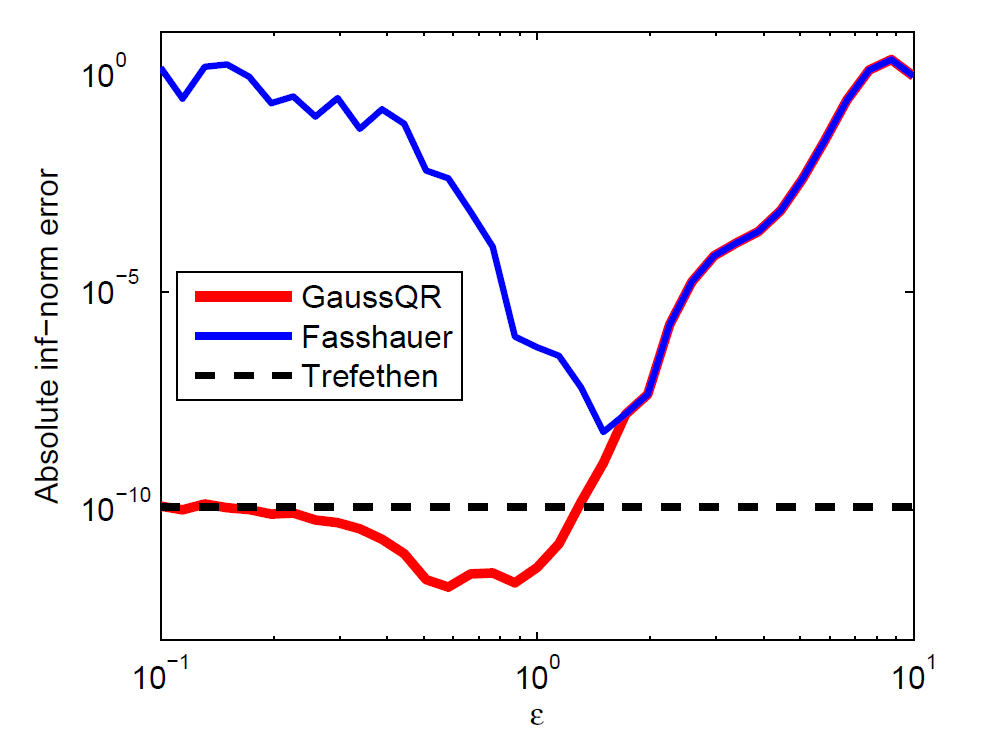
\includegraphics[height=2in]{HSSVD_BVP}
    \includegraphics[height=2in]{Fig_MFS_BEM}
\caption{Left: Comparison between use of the Hilbert--Schmidt SVD (GaussQR), standard kernel approach (Fasshauer) and Chebyshev polynomial spectral method (Trefethen) to solve a boundary value problem (from \citep{McCourt13}). Right: Cost per accuracy plot of several MFS solutions vs. BEM solution for coupled PDE system.}\label{Fig_MFS_BEM}
\end{figure}

As the next steps for this project we expect (i) to move to a head model that reflects the geometry of the brain more realistically, and (ii) to integrate the forward solver into a full inverse problem framework which will allow us to identify the locations of activity inside the brain from measurements of the electric potential (instead of simulating the electric surface potential based on a given dipole source as done for the forward problem in Fig.~\ref{Fig_MFS_BEM}).

\subsection*{Research Project 4.3. Using Kernels to Create a Surrogate Model to Predict the Spread of Ebola} \label{ebolasubsec}
Mike McCourt is working on a project titled ``Modeling the Ebola Epidemic with Discrete Time Filters'' at UC--Denver, where the DEXES II software (which was developed for the analysis, planning, and training for complex international humanitarian emergencies, peacekeeping missions, and non-traditional conflicts) is modified and then used to predict the state of the Ebola epidemic in West Africa within a data assimilation framework. A significant component of that work involves formalizing the mathematics of general discrete time filters, specifically the assimilation of data assumed to be Poisson distributed, and implementing such a Poisson filter efficiently in software. Key quantities of interest (QoI) include: the probability of any cases developing in Mali, the probability of a multimodal evolution within a region (after an initial peak is hit, can the disease regain momentum), or the total number of cases outside of presently infected regions.
As an extension of the modeling and predictive components of that project, we plan to study the effect of various input parameters for the DEXES II model on the evolution of the Ebola crisis.  Such parameters may include: border permeability (the probability that someone can enter a country without screening), the development of quarantines within a region, and the availability of clean water and waste disposal facilities.  If we think of QoI as a quantity of interest computed at the end of a predictive session, we may write QoI(permeability, quarantine, clean water) to denote the dependence of the QoI on a variety of model parameters.  As a result, studying the impact of these parameters on this QoI is a problem of surrogate modeling in potentially high dimensions.  Furthermore, as the number of dimensions we want to simultaneously consider increases, the experimental design for generating this surrogate model becomes increasingly relevant.  Thus, results from \refproba and \refprobcc should help with this Ebola study.

%\subsection*{Research Project 4.4. Low-rank Approximations for Kernel Classification}\label{Sec_TruncHS}
%
%One way to make support vector machines (SVMs) perform more efficiently is to consider a low-rank representation for the kernel as in \citep{FineScheinberg02}. We anticipate that we can use the eigenfunction expansion of $K$ to decrease the cost involved in the quadratic program required for the SVM solution. The standard SVM quadratic program can be written in matrix form as
%\begin{align}
%    \min_{\balpha} \;&
%        \frac{1}{2}\balpha^T\mD_{\by}\mK\mD_{\by}\balpha - \be^T\balpha \\
%    \text{subject to } & \by^T\balpha = 0, \nonumber\\
%    & \balpha\in[0,C]^N, \nonumber
%\end{align}
%where $\mD_{\by}$ is a diagonal matrix with $\by$ on the diagonal,
%and $\be$ is a vector of all ones.  By approximating the kernel matrix
%$\mK\approx(\mLambda^{1/2}\mPhi)^T(\mLambda^{1/2}\mPhi)$ using the matrices of kernel eigenvalues and eigenfunctions, $\mLambda$ and $\mPhi$, of \refproba we can rephrase this problem as
%\begin{align*}
%    \min_{\bnu,\balpha} \;&
%        \frac{1}{2}\begin{pmatrix}\bnu^T&\balpha^T\end{pmatrix}
%        \begin{pmatrix}\mI_M&0\\0&0\end{pmatrix}
%        \begin{pmatrix}\bnu\\\balpha\end{pmatrix}
%        - \begin{pmatrix}0&\be^T\end{pmatrix}\begin{pmatrix}\bnu\\\balpha\end{pmatrix} \\
%    \text{subject to } &
%        \begin{pmatrix}0&\by^T\\-\mI_M&\mLambda^{1/2}\mPhi^T\mD_{\by}\end{pmatrix}
%        \begin{pmatrix}\bnu\\\balpha\end{pmatrix} = 0, \nonumber\\
%    & \balpha\in[0,C]^N,\quad \bnu\in\reals^M. \nonumber
%\end{align*}
%Although
%this system is of size $N+M$ (and the original system was only size $N$), the
%cost of solving this system may be much lower because of the extremely simple
%structure of the Hessian.  This sparsity, in comparison to the Hessian for the exact kernel, which may be
%fully dense, allows for cheap matrix-vector products and decompositions, both
%of which may lead to a faster quadratic program solve.  Note that the $\bnu$
%values are inconsequential in making predictions with the SVM.
%
\section{Results of Previous NSF-Funded Research}\label{SectPrevious}

Greg Fasshauer (GEF) and Fred Hickernell (FJH) were the PIs for \emph{NSF-DMS-1115392 Kernel Methods for Numerical Computation}, July 1, 2011 -- June 30, 2014, \$320,000.  Since Fall 2005, we have organized a weekly Meshfree Methods research seminar that draws regular participation from all of our local collaborators, including faculty members, visitors, and students.  Participants take turns posing interesting research problems, reporting work-in-progress, and presenting relevant work of others.  The atmosphere is informal; interruption and discussion are encouraged.  Occasionally we have speakers from outside applied mathematics and/or IIT. Regular participants for a month or more during the timeframe of this project include the following ($\fF$ = female,  $\fA$ = African-American, $\fL$ = Latina/Latino).

\begin{description}[leftmargin=2.5ex]
\item[IIT Faculty] GEF, FJH, Igor Cialenco (IC), John Erickson (JE, $\fA$), Lulu Kang (LK, $\fF$);
\item[Visitors] Roberto Cavoretto (RC), U Torino; Sou-Cheng Choi (SCC, $\fF$), Research Assistant Professor, IIT, National Opinion Research Center, U Chicago; Salvatore Ganci (SG), U Palermo; YungWook Jung, Gyeonggi College of Science and Technology; Junbin Li, Dalian U Technology; Yiuwei Liu (YiL), Lanzhou U; Michael McCourt (MM), UC--Denver; Jinming Wu, Zhejiang Gongshang U;
\item[IIT Graduate Students] Aleks Borkovskiy (AB), Siyuan Deng (SD), Yuhan Ding (YD, $\fF$), Llu\'is Antoni Jim\'enez Rugama (LAJR), Lan Jiang (LJ, $\fF$), Yao Li (YaL), Yiou Li (YL, $\fF$), Jagadeeswaran Rathinavel (JR), Tiago Silva (TS), Xin Tong (XT, $\fF$), Qi Ye (QY), Xiaodong Zhang (XiZ), Yizhi Zhang (YZ), Xuan Zhou (XZ);
\item[IIT Undergraduate Students] Haocheng Bian (HB), Nick Clancy (NC), Martin Dillon (MD), Caleb Hamilton (CH), Joseph Kupiec, Barrett Leslie (BL), Timothy McCollam (TM), Martha Razo (MR, $\fL$, $\fF$);
\item[Other Undergraduate Students] Casey Bylund (CB, $\fF$), U San Francisco; Matthew Gliebe (MG), Northwestern U; Palmer Lao (PL), Clarkson U; William Mayner (WM), Brown U;
\item[High School Students] Sergey Papushin (SP), Sunny Yun (SY).
\end{description}

\subsection{Intellectual Merit from Previous NSF Funding}
\label{previousmeritsubsec}

With a collaborator we have investigated the convergence and tractability of meshfree methods, \eqref{rbfapprox}, using the Gaussian kernel with non-constant shape parameters, $\{\gamma_{\ell}\}_{\ell =1}^{\infty}$, \eqref{gausskernel}. Dimension-\emph{independent} convergence rates for function approximation were demonstrated, and they depend on the rate of decay of the $\gamma_{\ell}$ as $\ell \to \infty$, not on the smoothness of the kernel \citep{FasHicWoz12b, FasHicWoz12a}. These results were extended by XZ to a more general class of kernels that have a sequence of scale parameters $\{\alpha_{\ell}\}_{\ell=1}^{\infty}$ as well as shape parameters.  In this case the dimension-independent convergence rates depend on the rate of decay of the product $\alpha_{\ell} \gamma_{\ell}$ as $\ell \to \infty$ \citep{ZhoHic15a}.

Together with QY and other collaborators, we have shown how the optimal solution of problems posed on reproducing kernel Hilbert spaces can be extended to Banach spaces \citep{SonZhaHic12a, FasHicYe13a}.

Existing algorithms for multivariate or even infinite-dimensional approximation and integration problems require hand-tuning of the parameters that define the spaces of functions to which they apply, e.g., the shape or scale parameters of the associated reproducing kernel.  In our search for adaptive algorithms that automatically select these parameters, we started by looking for adaptive algorithms for even simpler problems. The adaptive algorithms that we developed are described below.  They all come with rigorous guarantees and are published in our Guaranteed Automated Integration Library (GAIL) \citep{ChoEtal14a}, which is publicly available and under ongoing development.

FJH, JL, YiL, and a collaborator developed an adaptive simple Monte Carlo algorithm for calculating means of random variables and multidimensional integrals \citep{HicEtal14a}.  This algorithm uses Cantelli's inequality to guarantee our estimate of the variance and uses a Berry--Esseen inequality (a finite sample Central Limit Theorem) to determine the necessary sample size.  Our adaptive algorithm is guaranteed to succeed for the cone of random variables or integrands whose kurtosis satisfies some known bound.  FJH and LAJR developed adaptive quasi-Monte Carlo cubature algorithms based on digital nets \citep{HicJim16a} and rank-1 integration lattices \citep{JimHic16a} by expressing the integrands as infinite series, $f=\sum_{\bk} \hatf_\bk \varphi_{\bk}$, where the $\varphi_{\bk}$ are Walsh functions or complex exponential functions.  The cubature error is bounded in terms of discrete  approximations to the coefficients, $\hatf_\bk$.  These algorithms must succeed for a cone of integrands whose true series coefficients do not decay erratically.

FJH, NC, YD, CH, and YZ constructed adaptive algorithms for univariate integration and function approximation \citep{HicEtal14b}.  This paper also sets out a general framework for constructing guaranteed adaptive algorithms for any problem where the solution operator is homogeneous by considering cones of input functions.  FJH, MR, and SY are preparing a paper that presents a new quadrature algorithm and explains these ideas to a broader audience.  XT completed her MS thesis \citep{Ton14a} on guaranteed adaptive optimization of univariate functions.

GEF and QY formulated a theory of generalized Sobolev spaces for reproducing kernel Hilbert spaces that connects kernel-based approximation methods to fundamental solutions of differential operators \cite{FasshauerYe11, FasshauerYe13}. An important contribution is the fact that the definition of these generalized Sobolev spaces involves both a notion of smoothness and of scale, while traditional Sobolev spaces take into account only the smoothness of functions in the space.
As an application of the generalized Sobolev space theory, GEF, QY and IC developed a framework for the numerical solution of stochastic partial differential equations with kernel-based methods \citep{CFY12,FasshauerYe13b,FasshauerYe14}.

GEF and MM developed the Hilbert--Schmidt SVD algorithm (sometimes also referred to as RBF-QR) for the stable computation with ``flat'' kernels as explained in \refproba. This approach takes advantage of the Hilbert--Schmidt series of the kernels \eqref{HSseries}. The basic framework was reported in a paper on stable computations with Gaussian kernels \citep{FMcC12}, and further extensions to the solution of boundary value problems for PDEs \citep{McCourt13}, a fast recursive regression algorithm \citep{McCourt13b}, and coupled PDE problems \citep{McCF14} have been submitted for publication. A publicly available library of \Matlab code \citep{McCFBG13} is under ongoing development.

A new class of \emph{iterated Brownian bridge kernels} was investigated by RC, GEF and MM \citep{CavorettoEtAl14}. The paper discusses these kernels, their connection to piecewise polynomial splines and an implementation of the associated Hilbert--Schmidt SVD algorithm. Special cases of these kernels were studied by CB and WM during their 2012 summer REU under the guidance of GEF and MM. During summer 2013, GEF and MM worked with two other undergraduate REU students, HB and MG, on the numerical computation of kernel eigenvalues and eigenfunctions (see \refprobab) and on an application of the Hilbert--Schmidt SVD to the study of the Hilbert space norm of the kernel interpolant. The latter problem is important for the error estimation of kernel-based methods, and for the determination of optimal kernel parameters (see \refprobc).

During SG's visit to IIT (08/2012--02/2013) he performed joint work with GEF and MM on the use of kernel-based methods for the solution of coupled boundary value problems for the application in EEG and MEG (see \refprobdb). This work makes use of the coupling framework of \cite{McCF14}. One joint paper is currently in press \citep{AFFGM15}, and \citep{AFFGM13} has been submitted.

Understanding the covariance kernel, eigenfunctions and associated Hilbert space of fractional Brownian motion was the focus of a research project during summer 2013 involving MD under the guidance of JE and GEF. Outcomes of this research were presented at the 2014 Joint Mathematics Meeting. During summer 2014 PL and TM looked at change of basis ways to overcome
the conditioning problems for kernel-based approximation
and collocation methods, and SP worked on optimal point configurations for kernel
interpolation under the guidance of JE and GEF.

\subsection{Broader Impacts from Previous NSF Funding}

We have trained a number of PhD, MS, BS, and high school students in research, as evidenced by the list above.  QY defended his PhD thesis in April 2012 and then became a Philip T. Church postdoc in the math department at Syracuse U. He has seven published papers, with one more each submitted and in preparation.  YL defended her thesis in August 2014 and is a visiting assistant professor at DePaul U.  Of the other nine IIT PhD students listed, YD, YL, XZ, and YZ have completed their comprehensive exams and are expected to graduate by the end of 2015.  AB has passed his qualifying exams.  LAJR, JR, TS, and XiZ are in the earlier stages of their PhD studies. SD, YaL, TS, XT, and XiZ completed their MS theses. The latter three are now PhD students.  QY, YD, LJ, LAJR, YL, XZ, HB, MR, SY, NC, MD, CH, BL, CB, WM, and SY have all presented their work at academic meetings in talks.

We have been pleased to have two underrepresented minority scientists and several female scientists (undergraduate through to faculty members) in our research group.  To their credit, both LJ and YL have successfully pursued their PhDs while at the same time carrying the responsibility of motherhood.

GEF presented a week-long tutorial to students from many different engineering disciplines at U Palermo. As a result, SG, a PhD student from Palermo supported by Italian funds, visited IIT from 08/2012-02/2013 to receive guidance on his research from GEF and MM.

RC, a postdoctoral researcher from U Torino supported by Italian funds, visited IIT from 03/2012-05/2012 and also in April 2013. He received advanced training in the area of meshfree approximation and has since been able to secure a position as a research fellow at U Torino.

Every fall semester in even years GEF teaches the graduate course MATH 590: Meshfree Approximation Methods, which focuses on kernel-based methods, and uses his monograph \citep{Fas07a} as a text. The new developments using eigenfunction expansions of positive definite kernels were integrated for the first time in fall 2012. GEF and MM have used the updated lecture notes of this course as a basis for a new book \citep{FMcC15}, currently under contract with World Scientific Publishers.

Every fall semester FJH teaches the graduate course MATH 565: Monte Carlo Methods in Finance.  The new results on adaptive (quasi-)Monte Carlo algorithms have been taught there since fall 2012, and the GAIL library is used by the students.

SCC and FJH offered an experimental graduate seminar course for seven students, MATH 573: Reliable Mathematical Software, during fall 2013. Our goal was to help computational mathematicians understand how to develop software that can be used by others.  Topics included guarantees for adaptive algorithms, reproducible computational science research, efficient coding, thorough documentation, careful testing, convenient user interfaces with parameter parsing and validation, and software publication.  We intend to offer this course again to an expanded audience because the topics are not normally covered in standard mathematics or computer science courses.

Members of the research team have organized conferences. Together with Larry L.~Schumaker, GEF organized the NSF-supported 14th International Conference on Approximation Theory in San Antonio, TX, in April 2013. A special mentoring session for PhD students and postdocs was included in the program of this conference. QY was the main organizer for the SIAM Student Chapter Conference on Recent Advances in Computational Science and Statistics held at IIT Oct. 29--30, 2011 (\href{http://www.math.iit.edu/~siam/workshop/}{\nolinkurl{www.math.iit.edu/~siam/workshop}}). BL was a co-organizer. This conference brought together graduate students and postdocs from various Chicago area universities and Argonne National Lab and featured three plenary lectures (by Jerry L. Bona, Charles K. Chui, and Wei B. Wu) along with 25 contributed talks and a poster session. Since then, other Chicago-Area SIAM chapters have joined the IIT chapter in organizing this conference on a yearly basis.

The research team has attended conferences, presented talks at departmental colloquia, and given talks to general audiences, both inside the mathematical sciences and beyond. Here are the highlights of the PIs.

%\begin{itemize}[leftmargin=2.5ex]
%\item
GEF gave minisymposium talks at the 2012, 2013, and 2014 SIAM Annual Meetings.  He also gave invited presentations at the Indiana-Illinois Workshop on Scientific Computing at Purdue U, April~2014, at the workshop on Multivariate Approximation and Interpolation with Applications in Erice, Italy in Sept.~2013, at the Freeform Optics Incubator Meeting of the Optical Society of America, Washington, D.C., in Oct.~2011, and at the NSF-CBMS Conference on Radial Basis Functions: Mathematical Developments and Applications, at UMass--Dartmouth, in June~2011. He gave a talk to the Level Set Collective at the NSF-sponsored Institute of Pure and Applied Mathematics (IPAM) and an invited talk at the 2013 Midwest Numerical Analysis Day. GEF is a steering committee member of the Midwest Numerical Analysis Conference series. In 2011, he gave a week-long workshop at U Palermo (Italy, engineering). GEF gave departmental colloquium/seminar talks at Chapman U (math \& computer science), U Chicago (statistics), Middle Tennessee State U (math), Northwestern U (industrial engineering \& management sciences), and U Padua (Italy, math).  GEF attended the 2010--2012 Intel International Science and Engineering Fairs (2011--2012 as chair of the AMS Menger Prize committee), where he judged projects in the mathematical sciences and interviewed high school students about their research. These interviews can be viewed on the YouTube channel of the AMS. He has also given presentations to students at Neuqua Valley and Carl Sandburg high schools.

%\item
FJH gave a talk at a special session at the 2012 Joint Mathematics Meetings (JMM), a plenary lecture at the Tenth International Conference on Monte Carlo and Quasi-Monte Carlo Methods in Scientific Computing (MCQMC) in 2012, an invited talk at the 2013 Midwest Numerical Analysis Day, and an invited session talk at the Eleventh MCQMC in April, 2014, an invited session talk at the 2014 SIAM Annual Meeting, and an invited talk at an ICERM workshop in September, 2014.  He spoke at the 2014 JMM and will speak at the 2015 JMM. FJH gave departmental colloquium/seminar talks at Argonne National Laboratory (mathematics and computer science), U Chicago (statistics), DePaul U (mathematics), Georgia Tech (industrial and systems engineering), and Illinois Institute of Technology (computer science, mathematics).  FJH was invited to speak to STEM students at Oakton Community College and to students at Hinsdale Central High School.

%\end{itemize}


\section{Broader Impact of Proposed Research}\label{SectBroad}


\subsection{Contributions to Training, Mentoring and Other Human Resource Developments}

The PIs, GEF and FJH, are dedicated to mentoring young researchers from high school through postdoctoral levels.  We are excited to see our mentees transition from curiosity about what scholarship entails to choosing and solving their own problems.  We are committed to our regular Meshfree Methods research seminar because we believe that we learn good research practices by seeing them modeled and we find good research ideas from a variety of sources. Outside of the Meshfree Methods seminar we meet with members individually or in smaller groups to discuss details of their research projects.

\begin{description}[leftmargin=0ex]
\item[Providing Research Experiences for Undergraduates and High School Students]\ We \linebreak[4]    strongly believe that students should be introduced to research before graduate school so that they can learn how to discover the unknown, something that is not taught well in a classroom. We request funds to support two summer REU students per year. Having advertised our REU opportunities for several years now has given us some visibility within the community and is prompting inquiries from prospective participants well before we even announce our latest program offerings. As in the past three years, we expect the NSF funds will serve as a catalyst for funds to support additional summer students. In choosing REU students we make a deliberate effort to build a diverse research environment by targeting female and underrepresented minority students as well as students from less research-focused institutions (see Sect.~\ref{SectPrevious}). We will also continue to receive well-prepared high school students to join our research group as we did for the past two summers.

\item[Preparing Students for Academic Careers] We consider mentoring to be a multi-faceted and potentially long-term process continuing even after the mentee has moved on from IIT.  For example, MM was an undergraduate student at IIT who collaborated with GEF during his PhD studies at Cornell U.  We will continue to mentor him as senior personnel for this proposal.
    %Similarly, although QY has left IIT, he has continued his collaboration with GEF and FJH.
    We have provided and will continue to provide SCC, a Research Assistant Professor at IIT and another senior personnel for this project, teaching and mentoring experience.  We will continue to find opportunities for special mentoring activities for our students, like those GEF organized and that QY and YD were involved in at the recent NSF-supported approximation theory conference in San Antonio.  We  will continue our collaboration with Argonne National Laboratory, which has led to short-term and long-term opportunities for our PhD students and graduates.

\item[Preparing Students for Industry Careers]
In addition to preparing students for the academic landscape, we also help current students land competitive jobs in the business world. The training we provide in the areas of algorithm development and coding tends to give our students the needed edge. For example, WM, who graduated from Brown U in May 2013, went on to work for an internet startup company.

\item[Supervising Visitors]
GEF has established contacts with several Italian universities attracting students and postdoctoral visitors to IIT for extended visits (see Sect.~\ref{SectPrevious}). Having lived in Hong Kong for 19 years, FJH has contacts with Chinese scientists that have prompted several long-term visiting Chinese scholars and students to join our research.  These activities will continue.

\item[Giving Short Courses and Invited Lectures]
We will continue our active track record (see Sect.~\ref{SectPrevious}) of providing lectures to students at various stages in their careers, ranging from high school to graduate school. These encourage students to enter STEM and encourage STEM students to engage in research.

\end{description}

\subsection{Contributions to Resources in Research, Education and the Broader Society}

The research we propose straddles mathematics, statistics, computer science, and applications in engineering and related fields.  The two PIs have complementary strengths that facilitate this interdisciplinary research.  GEF has expertise in approximation theory, meshfree methods, and numerical partial differential equations, while FJH has expertise in (quasi-)Monte Carlo methods, kernel-based methods, information-based complexity theory, and experimental design. Our expertise provides both an obligation and an opportunity to interact with a number of diverse communities. We envision the following contributions:

\begin{description}[leftmargin=0ex]
\item[Disseminating Research]
The research supported by this grant will result in publications in peer-reviewed journals in a broad spectrum of applied mathematics, computer science, statistics and engineering. These journals will include both those that emphasize theory and those that emphasize applications.

\item[Promoting Cones] The idea of guaranteed, adaptive algorithms via cones of input functions has broad potential application.  We will be promoting this idea among numerical analysts who develop new algorithms and analyze their computational costs, as well as among information-based complexity theorists who analyze the lower bounds on the complexity of numerical problems.

\item[Promoting the Hilbert--Schmidt SVD] Similarly, we will encourage other researchers to take advantage of the stability given to kernel-based methods by the Hilbert--Schmidt SVD, to use our code, and to join our research efforts. The paper \citep{FMcC12} has already received more than 40 citations on Google Scholar.

\item[Bridging Mathematics and Statistics]
This project touches on topics that are of interest to the statistics community: kriging, Monte Carlo methods, and design of experiments.  Historically, there has been relatively little interaction between numerical analysts and statisticians.  We have and will continue to engage the statistics community by speaking a their conferences and departmental seminars.  For example, in 2015 FJH will give a colloquium talk in the Department of Statistics at Virginia Tech and an invited talk at the $47^{\text{th}}$ Days of Statistics of the Soci\'et\'e Fran\c{c}aise de Statistique. The book \citep{FMcC15} by GEF and MM will contain several chapters bridging this gap.

\item[Collaborating with Engineers]
As a result of the visit by SG (see Sect.~\ref{SectPrevious}), GEF and MM have entered into an ongoing collaboration with engineering colleagues at U Palermo (see \refprobdb). We have submitted two separate joint proposals to the Italian government and to U Palermo to request support for this work (but without direct support for GEF and MM). Therefore, this collaboration will benefit from travel funds via the current proposal.
Since kernel methods are becoming a rather popular numerical tool in science and engineering, other opportunities for collaborations outside mathematics frequently arise. For example, GEF participated in an incubator meeting on freeform surfaces organized by the Optical Society of America.

\item[Promoting the Well-being of the Broader Society]
In \refprobdb kernel methods are being used for the solution of inverse problems arising in the detection of brain activity from MEG or EEG data. This fully non-invasive diagnostic procedure might help doctors detect early functional and neurophysiological markers of diseases (e.g., of Alzheimer's disease). It might also result in a potential reduction in doctors' visits, shorter hospitalization periods and a greater longevity with overall improved quality of life. Similarly, \refprobdc may provide insights that enable better management of the spread of the Ebola epidemic.

\item[Organizing and Presenting at Conferences]
We and our students involved in this project will present our results at a variety of conferences and workshops.  These include: (i) specialized meetings focusing on approximation theory, complexity, experimental design, meshfree methods, and Monte Carlo methods; (ii) the national meetings of AMS, SIAM, and the statistical societies; and (iii) conferences devoted to application areas.  We are frequently invited to speak at such conferences, which will give our results a prominent hearing. We will also continue to organize specialized conferences or minisymposia within larger conferences.

\item[Writing Textbooks and Survey Papers]
GEF and MM are currently under contract with \linebreak[4] World Scientific Publishers to prepare \citep{FMcC15}. This book will provide an exposition of the theory and implementation of the Hilbert--Schmidt SVD along with numerous applications. The book will form a bridge to the GaussQR library \citep{McCFBG13} currently under development and may serve as a textbook for a graduate class on meshfree methods, such as MATH 590 at IIT. GEF and FJH occasionally publish survey articles (e.g., a 42 page paper on kernel-based methods \citep{Fasshauer11}).

\item[Refreshing Course Syllabi]
MATH 590 (Meshfree Methods), taught by GEF in the fall semester of every even-numbered year, just underwent a major change as the preparation of \citep{FMcC15} progresses.
MATH 565 (Monte Carlo Methods in Finance), taught every fall by FJH, has incorporated our new results on guaranteed confidence intervals using IID or low discrepancy sampling. In the future it will include our new results on guaranteed multi-level and quasi-Monte Carlo sampling (see \refprobba).

Current texts teach students to estimate the error of the trapezoidal rule, $T_n(f)$, by $[T_n(f)-T_{n/2}(f)]/3$ (see, e.g., \cite[p.\ 223--224]{BurFai10}).  The arguments behind this estimate introduce the valuable concept of extrapolation, however, this is a flawed error estimate as pointed out $30$ years ago by James Lyness \cite{Lyn83} and highlighted by our recent work \cite{HicEtal14b}.  This same flawed idea underlies \Matlab's {\tt integral.m}.  We will urge numerical analysis textbook authors and educators to change the way that error estimation is taught based on our recent and proposed work.  These ideas will also enter our more traditional numerical analysis courses such as MATH 350 (Introduction to Computational Mathematics) or MATH 577 and 578 (Computational Mathematics I \& II).

\item[Creating Software and Collaborating with Software Developers]
GEF and MM have created the website \citep{McCFBG13} which serves as the home for the software on our stable algorithms built upon the Hilbert--Schmidt SVD. This \Matlab library is freely available and allows others to experiment with our code. Thus far, the library contains routines for Gaussian and iterated Brownian bridge kernels. As our research expands to other kernels and their eigenexpansions the resulting code will be added to the library. The GaussQR library also serves as a sandbox for students---especially REU students---to learn about our research and allows them to contribute pieces of their own work.
We will continue to develop GAIL \citep{ChoEtal14a} (now up to version 2) as part of our proposed research.  The GAIL software will serve the wider community that relies on numerical approximation and integration algorithms.  It will also demonstrate how adaptive algorithms ought to be implemented, which we hope will inspire and inform those working on adaptive algorithms for other mathematical problems.  We also expect our new algorithms to be incorporated into widely used numerical packages, as was done for our algorithm in \cite{HonHic00a} by \Matlab \citep{MAT8.4} and NAG \citep{NAG23}.  We will continue to discuss with software developers about these issues.

\item[Reaching Out]
GEF and FJH both have a record of reaching out to high school students and we plan to continue. The website \href{http://math.iit.edu/~openscholar/meshfree/}{\nolinkurl{math.iit.edu/~openscholar/meshfree/}} helps manage our internal and external communication and dissemination of research findings. Advertising for the summer REU experiences is also facilitated via this website.  Information about GAIL is at \href{http://code.google.com/p/gail}{\nolinkurl{code.google.com/p/gail}}.
\end{description}

\newpage
\clearpage
\pagenumbering{arabic}

\bibliographystyle{spbasic}

\renewcommand{\refname}{\hfill \textbf{\large References Cited} \hfill \hfill}                   %%
\renewcommand{\bibliofont}{\normalsize}

\bibliography{FJH22,FJHown23,GEF}
\end{document}
